\section{Géopolitique de la ville de Québec}\label{sec:geopolitique_quebec}
Cette section va faire un historique rapide de la géopolitique de la ville de Québec. Ceci est principalement pour dégager des grandes époques où les frontières sont restées stables et illustrer la complexité de représenter les règlements de plusieurs juridictions. \par
On observe trois grandes rafflées de fusions\parencite{VilledeQuebec:ReperesChronologique:}:
\begin{itemize}
  \item '65-'72:
  \SubItem{Duberger('70), Les Saules('70) et Neufchâtel ('71) rejoignent la ville de Québec}
  \SubItem{Ste-Foy et Ancienne Lorette fusionnent('70)}
  \SubItem{Le territoire de Wendake s'étend vers le Sud}
  \SubItem{Orsainville cède une péninsule de territoire à Charlesbourg}
  \SubItem{Beauport et Beauport-Ouest fusionnent('66)}
  \SubItem{Notre-Dame de Lorette devient L'Ancienne-Lorette('67)}
  \item '72-76:
  \SubItem{Charlesbourg, Orsainville, Charlesbourg-Est et Notre-Dame des Laurentides fusionnent pour devenir Charlesbourg ('76)}
  \SubItem{Charlesbourg-Ouest est annexé par Québec('76)}
  \SubItem{Giffard, Beauport, Courville, Villeneuve et Montmorency fusionnent('76) pour devenir Beauport}
  \SubItem{Val-Belair et Val-Saint-Michel fusionnent et deviennent Val-Belair('73)}
  \item '76-2001:
  \SubItem{Stabilité des limites territoriales}
  \item 2002:
  \SubItem{Fusion de Québec, L'Ancienne-Lorette, St-Augustin de Desmaures, Charlesbourg, Beauport, Val-Belair, Ste-Foy, St-Émile, Lac-St-Charles, Vanier, Cap-Rouge et Loretteville}
  \item 2006
    \SubItem{Séparation St-Augustin de Desmaures et L'Ancienne-Lorette}
\end{itemize}
\FloatBarrier
La figure \ref{fig:municipalites_carto_historique} montre l'évolution des barrières géopolitiques au cours du temps. 
\begin{figure}[ht]
  \centering
  \begin{subfigure}[t]{0.45\textwidth}
    \centering
    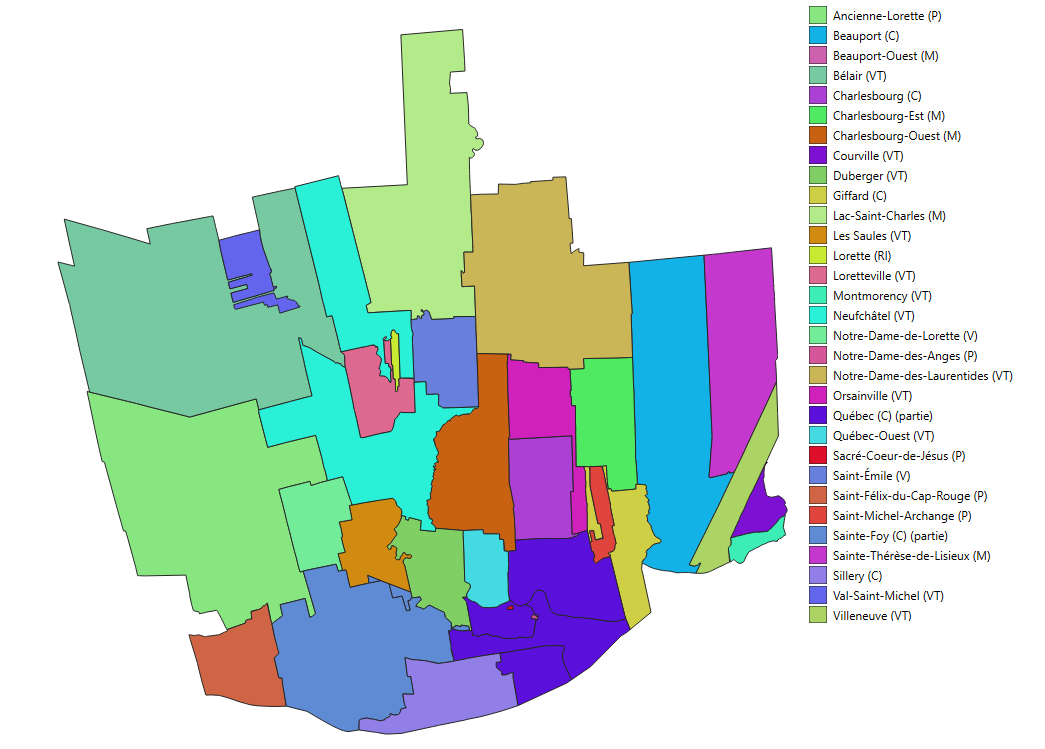
\includegraphics[width=0.9\linewidth]{images/municipalites_1965.png}
    \caption{1965}
    \label{fig:municipalites_1965}
  \end{subfigure}%
  \begin{subfigure}[t]{0.45\textwidth}
    \centering
    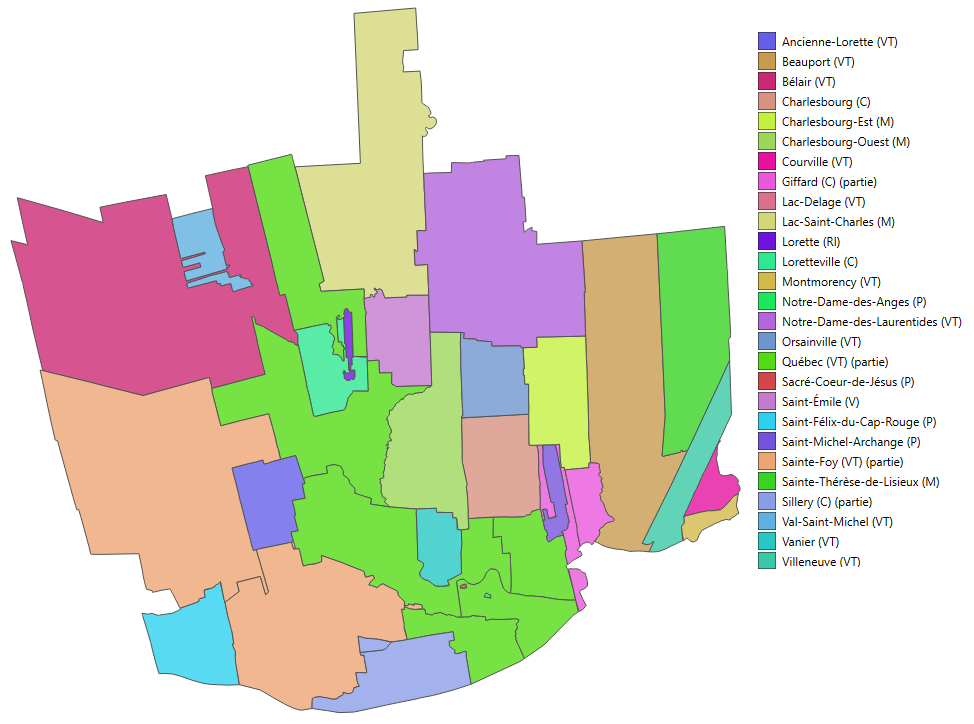
\includegraphics[width=0.9\linewidth]{images/municipalites_1972.png}
    \caption{1972}
    \label{fig:municipalites_1972}
  \end{subfigure}\\
  \begin{subfigure}[t]{0.45\textwidth}
    \centering
    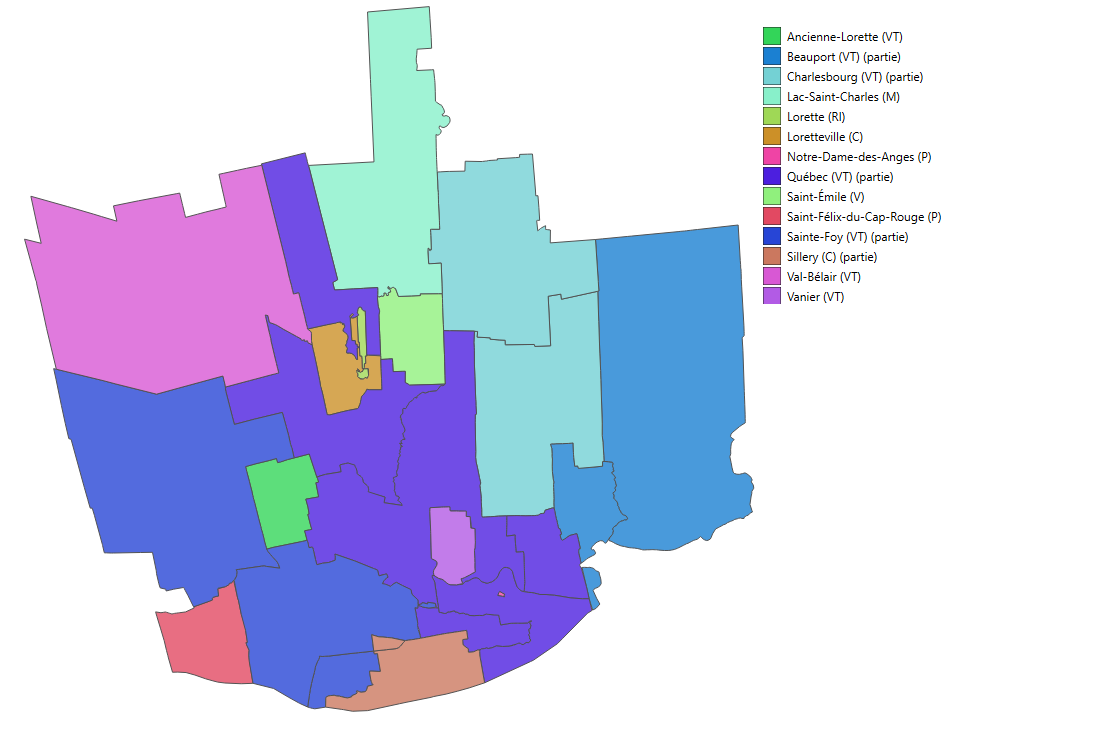
\includegraphics[width=0.9\linewidth]{images/municipalites_1980.png}
    \caption{1980}
    \label{fig:municipalites_1980}
  \end{subfigure}%
  \begin{subfigure}[t]{0.45\textwidth}
    \centering
    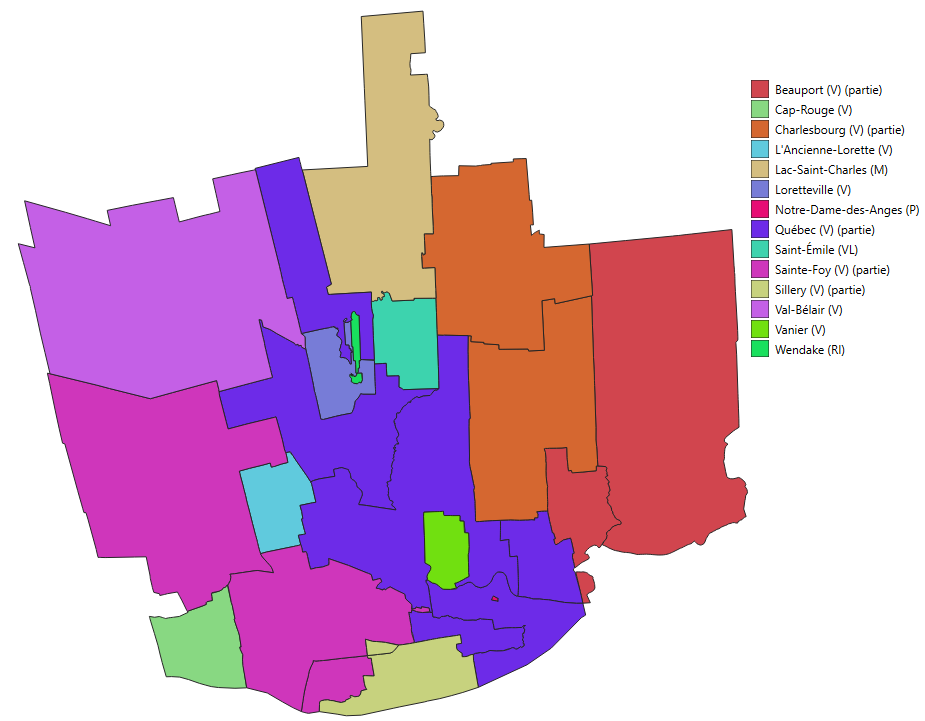
\includegraphics[width=0.9\linewidth]{images/municipalites_1988.png}
    \caption{1988}
    \label{fig:municipalites_1988}
  \end{subfigure}\\
  \begin{subfigure}[t]{0.45\textwidth}
    \centering
    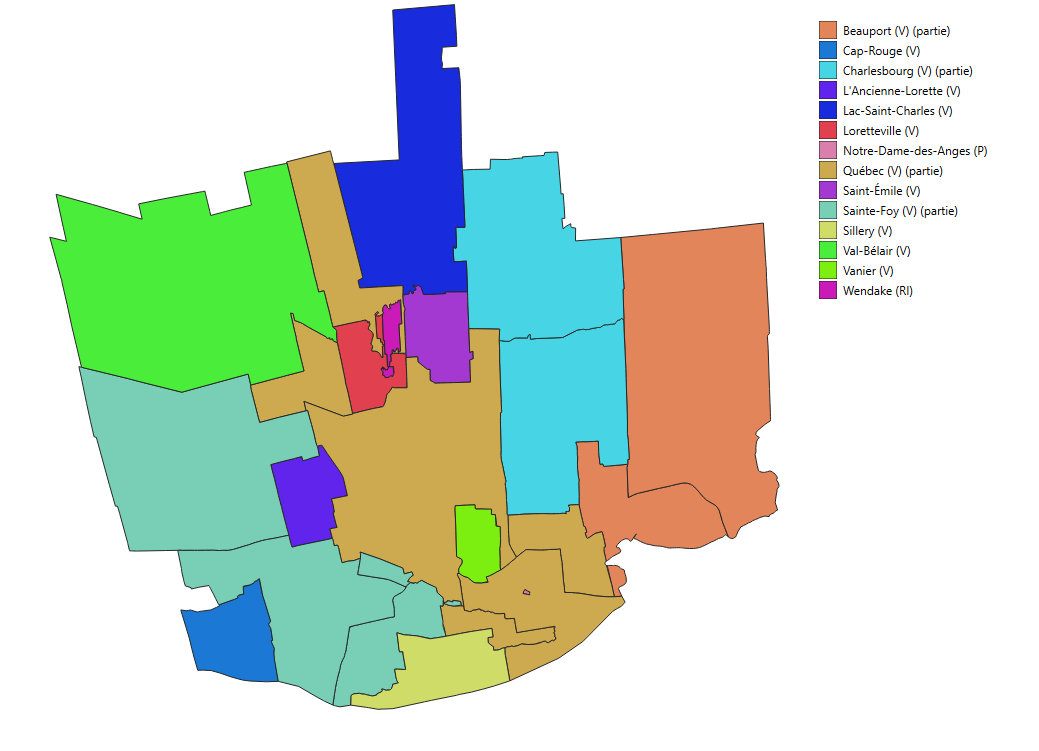
\includegraphics[width=0.9\linewidth]{images/municipalites_2001.png}
    \caption{2001}
    \label{fig:municipalites_2001}
  \end{subfigure}%
  \begin{subfigure}[t]{0.45\textwidth}
    \centering
    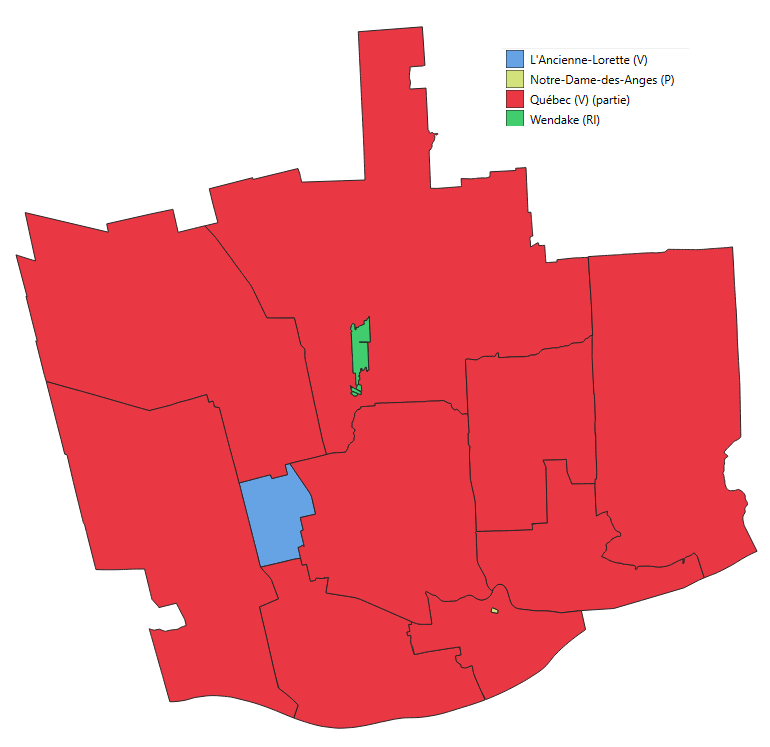
\includegraphics[width=0.8 \linewidth]{images/municipalites_2011.png}
    \caption{2011}
    \label{fig:municipalites_2011}
  \end{subfigure}%
  \caption{Séparation géopolitique du territoire de l'actuelle Ville de Québec \parencite{ElectionsQuebec:AtlasHistorique:2021}}\label{fig:municipalites_carto_historique}
\end{figure}

%Cela étant dit, l'historique de fusion de municipalités et la difficulté de trouver des codes d'urbanisme avant 1995 rend l'utilisation de ces données relativement difficile. La figure \ref{fig:historique_fusions} montre les fusions successives ayant mené à l'actuelle ville de Québec:
  %\begin{figure}[!h]
  %  \centering
  %  \captionsetup{justification=centering,margin=2cm}
  %  \includegraphics[width = 0.5\textwidth]{images/historique_fusions_VDQ.png}
  %  \captionsetup{justification=centering,margin=2cm}
  %  \caption{Diagramme montrant les fusions géopolitiques de la ville de Québec. \hl{Vérifier droits d'auteurs} Source: }
  %  \label{fig:historique_fusions}
  %\end{figure}
  %\FloatBarrier

%D'autre part, à travers les années '90, la ville de Québec va créer des requis de statinnement différents par quartiers. Post-fusion, les différentes villes garderont leurs codes d'urbanisme jusqu'en 2009 où la ville créera un code applicable à l'ensemble du territoire avec 4 sous zone: Général, Axe Structurant B, Axe Structurant A et Urbain Dense \parencite{VilledeQuebec:ReglementHarmonisation:2009}. La définition spatiale des unités de voisinage est donnée dans \textcite{VilledeQuebec:ZonageMunicipal:2024} et l'assignation de la zone est donnée dans \textcite{VilledeQuebec:GrilleSpecifications:2024}. La carte à la figure \ref{fig:types_unites_voisinage} montre les unités de voisinage pour la ville de Québec catégorisé selon la définition ci-haut:
\begin{figure}[ht]
  \centering
  \begin{subfigure}[t]{0.5\textwidth}
    \centering
    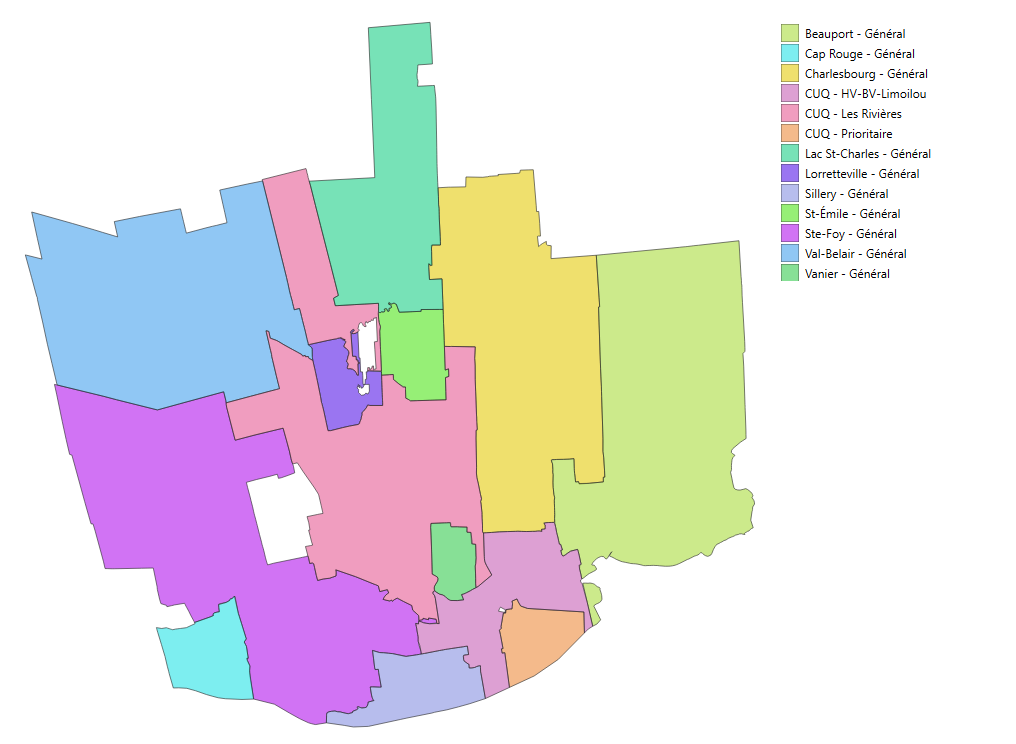
\includegraphics[width=0.9\linewidth]{images/geographie_code_urbanisme_1995-1997.png}
    \caption{1995-1997}
  \end{subfigure}~
  \begin{subfigure}[t]{0.5\textwidth}
    \centering
    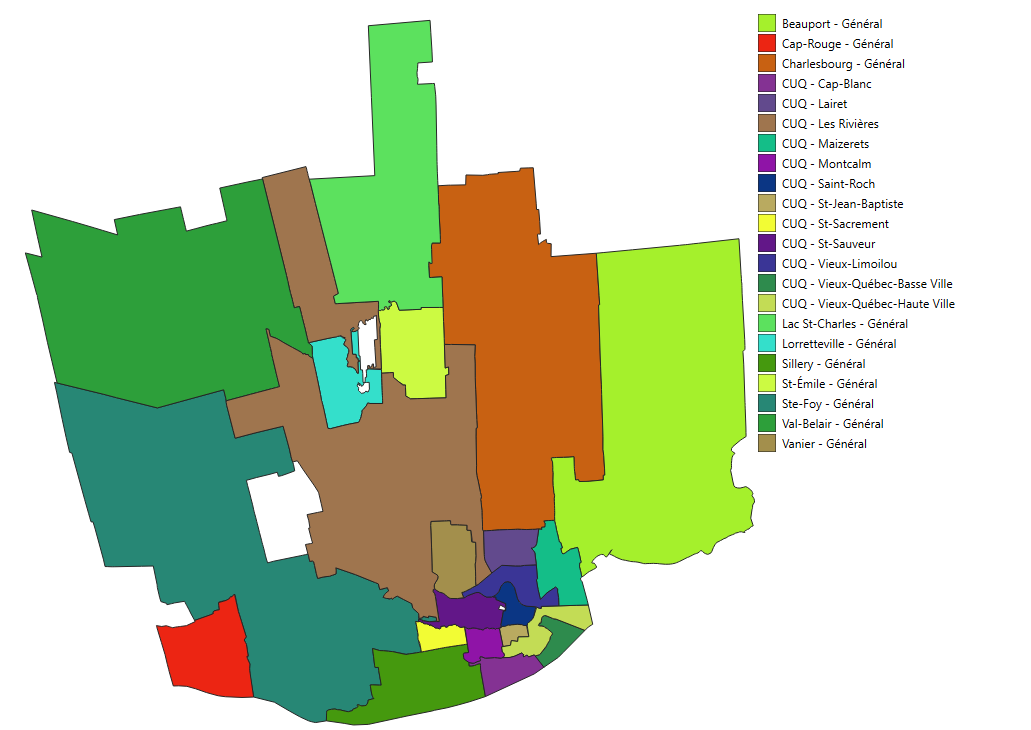
\includegraphics[width=0.9\linewidth]{images/geographie_code_urbanisme_1997-2009.png}
    \caption{1995-1997}
  \end{subfigure}\\
  \begin{subfigure}[t]{0.6\textwidth}
  \centering
  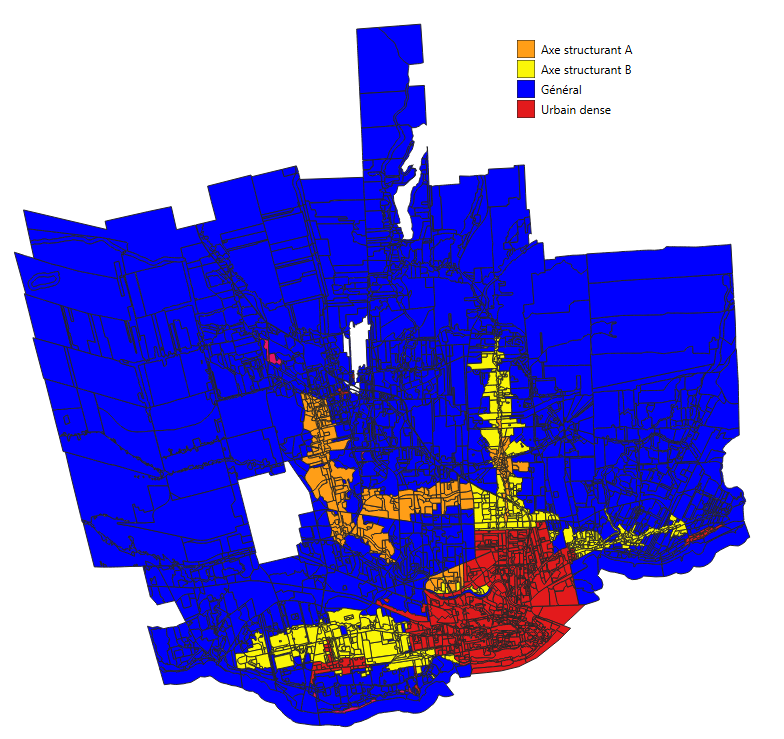
\includegraphics[width=0.8\linewidth]{images/geographie_code_urbanisme_2009_present.png}
  \caption{2010-présent}
  \end{subfigure}
  \caption{Secteur ayant des minimum de stationnement différents}
  \label{fig:types_unites_voisinage}
\end{figure}
\FloatBarrier
  


\section{Stationnement: politiques, couts et effets sur la mobilité}
  \subsection{Stationnement hors rue}
  Selon \textcite{Shoup:HighCost:2005}, les minimums de stationnement ont vu le jour dans les années 50 en réponse à la croissance du parc automobile et pour assurer que les commerçants et citoyens internalisaient les coûts associés à l'automobile. Ce mécanisme règlementaire est encore omniprésent au Québec puisque seuls les arrondissement de Côte des Neiges, du Sud-Ouest, du Plateau Mont-Royal et du Centre-Ville de Montréal \hl{besoin de citations}. La ville de Québec est en processus d'abroger ces requis pour l'habitation pour les zones en milieu dense ou le long des axes de transport en commun \parencite{VilledeQuebec:AdoptionReglement:2024}.\par
  En plus de l'hétérogénéité spatiale qui est décrite à la section \ref{sec:geopolitique_quebec}, on constate aussi une hétérogénéité au niveau des catégories utilisées pour les requis de stationnement. Ceci est d'autant plus ardu que les catégories utilisées dans les minimums de stationnement n'ont pas nécessairement d'équivalent direct dans le \ac{CUBF} utilisé dans le rôle foncier du Québec \parencite[Annexe 2C.1]{GouvernementduQuebec:ManuelEvaluation:2024}. Le tableau \ref{tab:req_stat_presents} et la figure \ref{fig:n_utilisation_CUBF_minimums} résument la présence d'un requis de stationnement explicité ou inféré pour un code \ac{CUBF} donné \parencite{VilledeQuebec:AdoptionReglement:2024,VilledeQuebec:ReglementZonage:1995}. Les codes d'urbanisme des municipalités pré-fusion sont issus d'un résumé fourni par la ville. Cette synthèse est nécessairement arbitraire: les catégories dans le codes d'urbanisme ne sont pas constantes entre les codes avec différents niveaux de superposition ou catégorisation par municipalité, rendant une synthèse difficile. La synthèse est recalé sur les codes \ac{CUBF} pour la simple raison que cette donnée sera exploité pour choisir la règlementation à appliquer pour inférer une capacité de stationnement requise. Les données sont issues d'une synthèse de la ville. Une demande a été complétée auprès du service de greffe pour obtenir les textes de loi.
  %\tiny
  \newcommand{\YCHECK}{\Checkmark}
  \newcommand{\NCHECK}{\cellcolor{red} \XSolid}
  \newcommand{\OCHECK}[1]{\cellcolor{orange} / #1}
  \newcolumntype{P}[1]{>{\centering\arraybackslash}p{#1}}
  \newcolumntype{M}[1]{>{\centering\arraybackslash}m{#1}}
  
  \setlength{\LTcapwidth}{\textwidth}
  \begin{landscape}
    \begin{center}
      \begin{longtable}{P{1.0cm} | p{7.5cm} | c || *{12}{P{5mm}}||p{6mm}} 
        \multirow{2}{*}{\STAB{\rotatebox[origin=c]{90}{Categ}}} & Juridiction & \STAB{\rotatebox[origin=c]{90}{Code \ac {CUBF}}} & \rotatebox[origin=c]{90}{  VDQ (2009-présent)} & \rotatebox[origin=c]{90}{VDQ (1995-2009)} & \rotatebox[origin=c]{90}{Beauport} & \rotatebox[origin=c]{90}{Cap-Rouge} & \rotatebox[origin=c]{90}{Charlesbourg} & \rotatebox[origin=c]{90}{Lac St-Charles} & \rotatebox[origin=c]{90}{Loretteville} & \rotatebox[origin=c]{90}{Sillery} & \rotatebox[origin=c]{90}{Ste-Foy} & \rotatebox[origin=c]{90}{St-Émile} & \rotatebox[origin=c]{90}{Val-Belair} & \rotatebox[origin=c]{90}{Vanier} & \rotatebox[origin=c]{90}{Nombre de requis} \\
        %& No. Règl. & MEFQ & R.V.Q. 1400 & V.Q.Z. 3 & 87-806 & 1151-95 & 96-2921 & 88-257 & 1386 & 950 & 3501 & 310-89 & VB-344-88 & 93-05-1245\\
        \hline  
        \endhead
        \hline
        \multicolumn{15}{c}{\Checkmark = Requis présent, \colorbox{red}{\XSolid} = Requis absent, \colorbox{orange}{/} = Requis implicite à une définition plus générale}\\\hline
        \endfoot
        \hline
        \multicolumn{15}{c}{\Checkmark = Requis présent, \colorbox{red}{\XSolid} = Requis absent, \colorbox{orange}{/} = Requis implicite à une définition plus générale}\\\hline
        \caption{Présence de règlementation de stationnement selon le code \ac{CUBF}}\label{tab:req_stat_presents}
        \endlastfoot
        \multirow{6}{*}{\STAB{\rotatebox[origin=c]{90}{Résidentiel}}} & Logement & 10XX & \YCHECK & \YCHECK &\YCHECK & \YCHECK &\YCHECK &\YCHECK& \YCHECK & \YCHECK & \YCHECK &\YCHECK & \YCHECK & \YCHECK&12\\
        & Logement subventionné & 10XX & \YCHECK & \YCHECK & \NCHECK & \NCHECK & \NCHECK& \NCHECK &\NCHECK &\NCHECK &\NCHECK &\NCHECK &\NCHECK & \NCHECK&2 \\
        & Habitation Collectives & 15XX & \YCHECK & \NCHECK & \YCHECK & \YCHECK & \YCHECK & \YCHECK & \YCHECK & \NCHECK & \NCHECK & \YCHECK & \YCHECK & \NCHECK&8 \\
        & Maison de chambres &  151X & \YCHECK & \YCHECK & \OCHECK{} & \OCHECK{} & \OCHECK{} & \OCHECK{} & \YCHECK & \NCHECK & \YCHECK &\OCHECK{} & \YCHECK & \YCHECK&6\\
        & Maison de retraite non autonomes & 1541 & \OCHECK{} & \YCHECK & \YCHECK & \YCHECK & \OCHECK{} & \OCHECK{} & \YCHECK & \YCHECK & \YCHECK & \OCHECK{} & \OCHECK{} & \NCHECK &6\\
        & Maison de retraite autonomes & 1543 & \OCHECK{} & \YCHECK & \YCHECK & \YCHECK & \OCHECK{} & \OCHECK{} & \YCHECK & \YCHECK & \YCHECK & \OCHECK{} & \OCHECK{} & \NCHECK&6 \\ 
        \hline
        \multirow{7}{*}{\STAB{\rotatebox[origin=c]{90}{Industriel / Infra.}}}& Industriel Général & \makecell[l]{2XXX\\3XXX} & \YCHECK & \YCHECK & \YCHECK & \YCHECK & \YCHECK & \YCHECK & \YCHECK & \YCHECK & \YCHECK & \YCHECK & \YCHECK & \YCHECK&12 \\
        & Industrie Haute Technologie & \makecell[l]{355X\\356X\\357X} & \YCHECK & \OCHECK{} & \OCHECK{}  & \OCHECK{}  & \OCHECK{}   & \OCHECK{}   & \OCHECK{}   & \OCHECK{}   &  \YCHECK & \OCHECK{}   & \OCHECK{}& \OCHECK{}&2 \\
        & Industrie mise en valeur et récupération &487X & \YCHECK & \OCHECK{} & \OCHECK{} & \OCHECK{} & \OCHECK{} & \OCHECK{} & \OCHECK{} & \OCHECK{} & \YCHECK & \OCHECK{} & \OCHECK{} & \OCHECK{}&2 \\ 
        & Entreposage & 637X & \YCHECK&\YCHECK&\OCHECK{}&\OCHECK{}&\OCHECK{}&\OCHECK{}&\YCHECK&\YCHECK&\OCHECK{}&\YCHECK&\YCHECK&\YCHECK &7\\
        & Service de construction & 66XX & \OCHECK{}  & \OCHECK{} &\OCHECK{} &\OCHECK{} &\OCHECK{} &\OCHECK{} & \YCHECK &\OCHECK{} &\OCHECK{} & \OCHECK{} & \OCHECK{} & \YCHECK&2\\
        \hline
        \multirow{4}{*}{\STAB{\rotatebox[origin=c]{90}{Commerces}}} & Centre et Immeuble Commercial & 50XX & \YCHECK & \YCHECK & \YCHECK & \YCHECK &\YCHECK&\YCHECK& \YCHECK&\YCHECK&\YCHECK&\YCHECK&\YCHECK&\YCHECK&12\\
        & Vente en gros & 51XX &\OCHECK{}&\YCHECK&\OCHECK{}&\OCHECK{}&\OCHECK{}&\OCHECK{}&\YCHECK&\OCHECK{}&\OCHECK{}&\OCHECK{}&\YCHECK&\OCHECK{}&3\\
        & Vente au détail construction et quincaillerie & 52XX&\OCHECK{}&\OCHECK{}&\OCHECK{}&\YCHECK&\OCHECK{}&\OCHECK{}&\YCHECK&\YCHECK&\YCHECK&\OCHECK{}&\YCHECK&\OCHECK{}&5 \\
        & Vente au détail marchandises & 53XX&\OCHECK{}&\OCHECK{}&\OCHECK{}&\OCHECK{}&\OCHECK{}&\OCHECK{}&\OCHECK{}&\OCHECK{}&\OCHECK{}&\OCHECK{}&\OCHECK{}&\OCHECK{}&0\\
        \multirow{6}{*}{\STAB{\rotatebox[origin=c]{90}{Commerces}}} & Vente au détail de l'alimentation & 54XX &\YCHECK&\YCHECK&\OCHECK{}&\OCHECK{}&\YCHECK&\YCHECK&\YCHECK&\YCHECK&\YCHECK&\YCHECK&\YCHECK&\YCHECK &10\\
        & Vente au détail de véhicules et produits connexes & 55XX &\YCHECK&\OCHECK{}&\OCHECK{}&\OCHECK{}&\OCHECK{}&\YCHECK&\YCHECK&\YCHECK&\YCHECK&\YCHECK&\YCHECK&\YCHECK&8\\
        & Station Essence & 553X&\YCHECK&\YCHECK&\YCHECK&\OCHECK{}&\OCHECK{}&\OCHECK{}&\YCHECK&\OCHECK{}&\YCHECK&\YCHECK&\YCHECK&\YCHECK&7 \\
        & Vente au détail de vêtements & 56XX&\OCHECK{}&\OCHECK{}&\OCHECK{}&\OCHECK{}&\OCHECK{}&\OCHECK{}&\YCHECK&\OCHECK{}&\YCHECK&\OCHECK{}&\OCHECK{}&\OCHECK{}&2\\
        & Vente au détail de mobilier & 57XX&\YCHECK&\YCHECK&\OCHECK{}&\OCHECK{}&\OCHECK{}&\OCHECK{}&\YCHECK&\OCHECK{}&\OCHECK{}&\OCHECK{}&\OCHECK{}&\OCHECK{}&3 \\
        & Vente au détail Autre & 59XX&\OCHECK{}&\OCHECK{}&\OCHECK{}&\OCHECK{}&\OCHECK{}&\OCHECK{}&\OCHECK{}&\OCHECK{}&\OCHECK{}&\OCHECK{}&\OCHECK{}&\OCHECK{}&0\\
        \hline
        \multirow{7}{*}{\STAB{\rotatebox[origin=c]{90}{Restaurants et bars}}} & Restaurant & 581X & \YCHECK&\NCHECK&\YCHECK&\NCHECK&\YCHECK&\YCHECK&\YCHECK&\YCHECK&\YCHECK &\YCHECK&\YCHECK&\YCHECK&7 \\
        & Restaurant plein service & \makecell{5811 \\ 5812 \\ 5815}& \OCHECK{}&\YCHECK&\OCHECK{}&\YCHECK&\OCHECK{}&\OCHECK{}&\OCHECK{}&\OCHECK{}&\OCHECK{}&\OCHECK{}&\OCHECK{}&\OCHECK{}&2\\
        & Restaurant service restreint/libre service& \makecell{5811 \\ 5812 }& \OCHECK{}&\YCHECK&\OCHECK{}&\YCHECK&\OCHECK{}&\OCHECK{}&\OCHECK{}&\OCHECK{}&\OCHECK{}&\OCHECK{}&\OCHECK{}&\OCHECK{}&2\\
        & Débit d'alcool & 582X&\YCHECK&\YCHECK&\YCHECK&\YCHECK&\YCHECK&\YCHECK&\YCHECK&\YCHECK&\YCHECK&\YCHECK&\YCHECK&\YCHECK&11\\
        \hline
        \multirow{3}{*}{\STAB{\rotatebox[origin=c]{90}{Tourisme}}} & Établissement d'hébergement & 583X&\YCHECK&\NCHECK&\NCHECK&\YCHECK&\YCHECK&\YCHECK&\YCHECK&\YCHECK&\YCHECK&\YCHECK&\YCHECK&\YCHECK&10\\
        & Hôtel & 5831&\OCHECK{}&\YCHECK&\YCHECK&\OCHECK{}&\OCHECK{}&\OCHECK{}&\OCHECK{}&\OCHECK{}&\OCHECK{}&\OCHECK{}&\OCHECK{}&\OCHECK{}&2\\
        & Môtel & 5832&\OCHECK{}&\YCHECK&\YCHECK&\OCHECK{}&\OCHECK{}&\OCHECK{}&\OCHECK{}&\OCHECK{}&\OCHECK{}&\OCHECK{}&\OCHECK{}&\OCHECK{}&2\\
        \hline
        & Services & 6XXX & \YCHECK & \YCHECK & \YCHECK &\YCHECK & \YCHECK & \YCHECK & \YCHECK & \YCHECK &\YCHECK &\NCHECK &\YCHECK&\NCHECK&10\\
        & Immeubles à bureaux & 60XX&\YCHECK&\YCHECK&\OCHECK{}&\YCHECK&\YCHECK&\YCHECK&\YCHECK&\YCHECK&\YCHECK&\NCHECK&\YCHECK&\NCHECK&9\\
        \multirow{19}{*}{\STAB{\rotatebox[origin=c]{90}{Services}}}& Finance, Assurance et Service immobilier & 61XX&\OCHECK{}&\YCHECK&\OCHECK{}&\OCHECK{}&\OCHECK{}&\OCHECK{}&\YCHECK&\OCHECK{}&\OCHECK{}&\YCHECK&\OCHECK{}&\YCHECK&4\\
        & Banque & 611X&\OCHECK{}&\YCHECK&\OCHECK{}&\YCHECK&\OCHECK{}&\YCHECK&\YCHECK&\YCHECK&\YCHECK&\OCHECK{}&\YCHECK&\OCHECK{}&7\\
        & Service personnels & 62XX & \OCHECK{} &\OCHECK{}&\OCHECK{}&\OCHECK{}&\YCHECK&\OCHECK{}& \OCHECK{}&\OCHECK{}&\YCHECK&\OCHECK{} &\OCHECK{}&\OCHECK{}&2\\
        & Salon de beauté / coiffure& 623X& \OCHECK{}&\YCHECK&\OCHECK{}&\OCHECK{}&\OCHECK{}&\OCHECK{}&\YCHECK&\OCHECK{}&\OCHECK{}&\OCHECK{}&\OCHECK{}&\YCHECK &3\\
        & Salon funéraire& 624X&\YCHECK&\YCHECK&\YCHECK&\YCHECK&\YCHECK&\YCHECK&\YCHECK&\YCHECK&\YCHECK&\YCHECK&\YCHECK&\YCHECK&12\\
        & Services d'affaires & 63XX &\OCHECK{}&\OCHECK{}&\YCHECK&\OCHECK{}&\OCHECK{}&\OCHECK{}&\YCHECK&\OCHECK{}&\OCHECK{}&\YCHECK&\OCHECK{}&\YCHECK&4\\
        & Services de réparation & 64XX&\OCHECK{}&\OCHECK{}&\OCHECK{}&\OCHECK{}&\OCHECK{}&\OCHECK{}&\OCHECK{}&\OCHECK{}&\OCHECK{}&\OCHECK{}&\OCHECK{}&\OCHECK{}&0\\
        & Service de réparation d'automobiles&641X&\YCHECK&\YCHECK&\YCHECK&\YCHECK&\OCHECK{}&\OCHECK{}&\YCHECK&\OCHECK{}&\YCHECK&\YCHECK&\YCHECK&\YCHECK&9\\
        & Service de réparation de mobiliers, d'équipements et de machines & 642X&\OCHECK{}&\OCHECK{}&\OCHECK{}&\OCHECK{}&\OCHECK{}&\OCHECK{}&\YCHECK&\OCHECK{}&\OCHECK{}&\OCHECK{}&\OCHECK{}&\OCHECK{}&1\\ 
        & Service de réparation de véhicules légers& 643X&\YCHECK&\YCHECK&\YCHECK&\YCHECK&\OCHECK{}&\OCHECK{}&\YCHECK&\OCHECK{}&\YCHECK&\YCHECK&\YCHECK&\YCHECK&9\\
        & Service de réparation et d'entretien de véhicules lourds& 644X&\YCHECK&\YCHECK&\YCHECK&\YCHECK&\OCHECK{}&\OCHECK{}&\YCHECK&\OCHECK{}&\YCHECK&\YCHECK&\YCHECK&\YCHECK&9\\
        & Service professionnel & 65XX&\YCHECK&\OCHECK{}&\YCHECK&\YCHECK&\OCHECK{}&\OCHECK{}&\OCHECK{}&\OCHECK{}&\OCHECK{}&\OCHECK{}&\OCHECK{}&\OCHECK{}&0\\
        & Service médical et de santé & 651X&\YCHECK&\YCHECK&\OCHECK{}&\OCHECK{}&\YCHECK&\YCHECK&\YCHECK&\YCHECK &\YCHECK & \OCHECK{} &\YCHECK & \OCHECK{}&9\\
        & Service d'hôpital & 6513 &\YCHECK &\YCHECK &\YCHECK &\YCHECK&\YCHECK&\YCHECK&\YCHECK&\YCHECK&\YCHECK&\YCHECK&\YCHECK&\YCHECK&12\\
        & Sanatorium, maison de convalescence et de repos & 6516 &\YCHECK &\YCHECK &\YCHECK&\OCHECK{}&\YCHECK &\YCHECK&\YCHECK&\YCHECK&\YCHECK&\YCHECK&\YCHECK&\YCHECK&11\\
        \multirow{12}{*}{\STAB{\rotatebox[origin=c]{90}{Services}}}& Service gouvernemental&67XX&\OCHECK{} & \OCHECK{} &\OCHECK{}&\OCHECK{}&\OCHECK{} &\OCHECK{} & \YCHECK&\OCHECK{}&\YCHECK&\YCHECK&\YCHECK&\YCHECK &5 \\
        & Pompiers/Police &672X&\YCHECK & \YCHECK &\OCHECK{}&\OCHECK{} &\OCHECK{} & \OCHECK{}&\OCHECK{}&\YCHECK&\OCHECK{}&\YCHECK&\OCHECK{}&\OCHECK{}&4\\
        & Service éducationnel&68XX&\YCHECK&\YCHECK&\NCHECK&\YCHECK&\NCHECK&\YCHECK&\YCHECK&\YCHECK&\NCHECK&\YCHECK{}&\YCHECK&\YCHECK &9 \\
        & Service de garderie&6541&\YCHECK&\OCHECK{}&\OCHECK{}&\OCHECK{}& \YCHECK&\OCHECK{}& \YCHECK &\OCHECK{}&\YCHECK&\OCHECK{}&\YCHECK&\OCHECK{}&5 \\
        & École Maternelle&6811&\OCHECK{}&\OCHECK{}&\OCHECK{}&\OCHECK{}&\OCHECK{}&\OCHECK{}&\YCHECK&\OCHECK{}&\YCHECK&\OCHECK{}&\YCHECK{}&\YCHECK{}&4 \\
        & École Primaire&6812&\YCHECK&\YCHECK&\YCHECK&\YCHECK&\YCHECK&\YCHECK&\YCHECK&\YCHECK&\YCHECK&\OCHECK{}&\YCHECK&\YCHECK&11 \\
        & École Secondaire / Polyvalente&\makecell{6813\\6822}&\YCHECK&\YCHECK&\YCHECK&\OCHECK{}&\YCHECK& \YCHECK&\YCHECK&\YCHECK&\YCHECK&\OCHECK{}&\YCHECK&\YCHECK&10 \\
        & CÉGEP &6823&\YCHECK&\YCHECK&\YCHECK&\OCHECK{}&\OCHECK{}&\YCHECK&\YCHECK&\OCHECK{}&\YCHECK&\OCHECK{}&\OCHECK{}&\OCHECK{}&6\\
        & Université&6821&\YCHECK&\YCHECK&\YCHECK&\OCHECK{}&\YCHECK&\YCHECK&\YCHECK&\OCHECK{}&\YCHECK&\OCHECK{}&\OCHECK{}&\OCHECK{}&7\\ 
        & Services religieux &691X&\YCHECK&\OCHECK{}&\YCHECK&\YCHECK&\OCHECK{}&\YCHECK&\YCHECK&\YCHECK&\YCHECK&\OCHECK{}&\YCHECK&\YCHECK&9\\
        \hline
        \multirow{8}{*}{\STAB{\rotatebox[origin=c]{90}{Culture et Récréation}}} & Culture, Récréation et Loisirs&7XXX &\NCHECK&\YCHECK&\YCHECK&\NCHECK&\YCHECK&\YCHECK&\NCHECK&\YCHECK&\NCHECK&\YCHECK&\YCHECK&\YCHECK&8\\
        & Activité Culturelle(Musée, Biblio) &711X&\YCHECK&\YCHECK&\YCHECK&\YCHECK&\YCHECK&\YCHECK&\YCHECK&\YCHECK&\YCHECK &\OCHECK{} &\OCHECK{} &\OCHECK{}&9\\
        & Assemblée de loisirs(Théâtre, Cinéma) &721X&\YCHECK&\YCHECK&\YCHECK& \YCHECK& \YCHECK&\YCHECK&\YCHECK&\YCHECK&\YCHECK&\OCHECK{}&\YCHECK&\OCHECK{}&10 \\
        & Installation sportive (Stade, Hippodrome)&722X&\YCHECK&\OCHECK{}&\OCHECK{}&\NCHECK&\OCHECK{}&\OCHECK{}&\YCHECK&\OCHECK{}&\YCHECK&\OCHECK{}&\OCHECK{}&\OCHECK{}&3\\
        & Centre de congrès&723X& \OCHECK{} & \YCHECK & \OCHECK{} & \NCHECK & \OCHECK{} & \OCHECK{}& \YCHECK& \OCHECK{} & \OCHECK{} & \OCHECK{} & \OCHECK{} & \OCHECK{}&2 \\
        & Activités récréatives&74XX&\YCHECK&\OCHECK{}&\YCHECK&\NCHECK&\OCHECK{}&\OCHECK{}&\YCHECK&\OCHECK{}&\YCHECK&\OCHECK{}&\OCHECK{}&\OCHECK{} &4\\
        & Terrains de golf&\makecell{7411\\7412}& \YCHECK& \OCHECK{}&\OCHECK{}&\NCHECK&\OCHECK{}&\OCHECK{}&\YCHECK&\OCHECK{}&\YCHECK&\YCHECK&\OCHECK{}&\OCHECK{}&4\\
        & Arena& 7451& \YCHECK&\YCHECK&\OCHECK{}&\NCHECK&\OCHECK{}&\OCHECK{}&\YCHECK{}&\YCHECK&\OCHECK{}&\YCHECK&\YCHECK&\OCHECK{}&6\\
        & Parcs/Camps &\makecell{75XX\\76XX}&\YCHECK &\NCHECK&\NCHECK&\NCHECK&\NCHECK&\NCHECK&\NCHECK&\NCHECK&\YCHECK&\YCHECK&\NCHECK&\YCHECK&5 \\
        \hline
        N/A & Extraction de ressources / Agriculture & 8XXX&\YCHECK&\NCHECK&\NCHECK&\NCHECK&\NCHECK&\NCHECK&\YCHECK&\NCHECK&\YCHECK&\NCHECK&\NCHECK&\NCHECK&3\\
      \end{longtable}
    \end{center}  
    \begin{figure}[h]
      \centering
      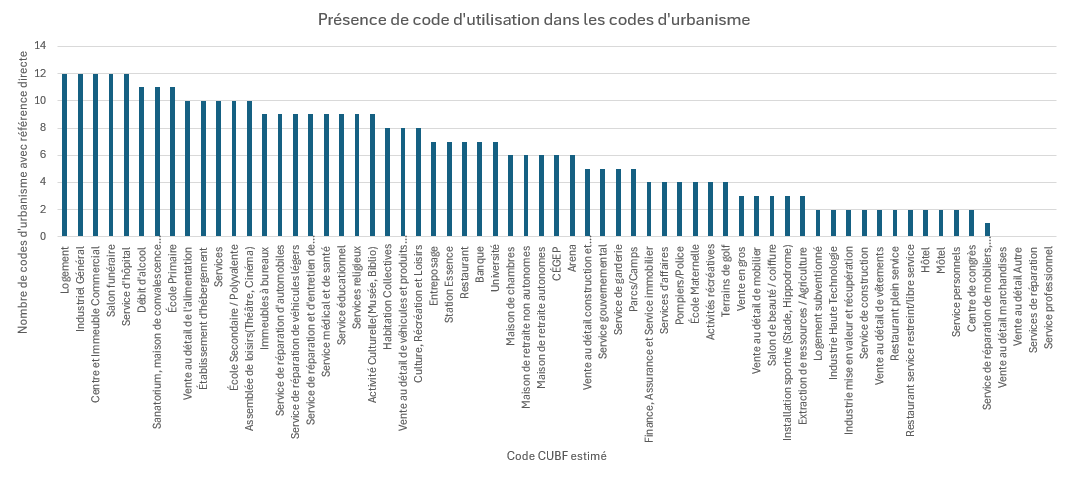
\includegraphics[width=22cm]{images/presence_requis_par_CUBF}
      \caption{Nombre de codes d'urbanisme utilisant les codes d'utilisation listés}\label{fig:n_utilisation_CUBF_minimums}
    \end{figure}
  \end{landscape}
  %\normalsize
  \FloatBarrier
  
  Les objets sur lesquels sont basés les codes d'urbanisme sont aussi hétérogènes. Bien que la plupart des requis soient basé sur une surface de plancher, certains sont exprimés en fonction d'autres objets considérés pertinents. D'autre part, la même utilisation du sol n'est pas nécessairement légiférée en utilisant le même objet entre deux juridictions différentes. Le tableau \ref{tab:objet_pour_inference_capacite} synthétise les objets considérés et les usages pour lesquels ils sont utilisés.

  \begin{table}[h]
    \centering
    \begin{tabular}{p{4cm} p{8cm}}
      \hline
      Objets considéré & Usages pertinents \\
      \hline
      Superficie de plancher & Majoritaire\\
      Superficie par usage (bureau, plateau TV) & Station télé \\
      Superficie de terrain & parc, zoo \\
      Logement & Logement \\
      Chambres & Maison de chambres, hébergement touristique, établissement de santé\\
      Lit & Établissement de santé, auberges de jeunesse, établissement carcéral \\
      Baie de service & Commerces liés à l'automobile\\
      Siège & Lieux de rassemblement, cinéma, théâtres, stades \\
      Salle & Cabinet médical, établissement scolaire, salon funéraire\\
      Personne & Débit d'alcool\\
      Employé & Services et vente au détail\\
      Médecin & Établissement de santé\\
      Étudiant & Établissement scolaire\\
      Plateau sportif & Golf, tennis, quilles, billards\\
      Poste de travail & Services personnels (salon de beauté)\\
      \hline
    \end{tabular}
    \caption{Récapitulatif des objets considérés pour fixer les capacité de stationnement}\label{tab:objet_pour_inference_capacite}
  \end{table}
  

  \FloatBarrier
  \subsection{Coûts de provision}
    Plusieurs coûts sont associés à la provision de stationnements, autant pour les individus, que pour les collectivités locales ou de tierces parties plus difficiles à identifier dans le cas d'externalités. Cette section visera à identifier quels sont les coûts associés et qui les porte.

    \subsubsection{Propriétaires fonciers et municipalités}
      \textcite{Blanc:EffectsUrban:2014} ont estimé la valeur foncière de 6 villes américaines en évaluant la valeur foncière des bâtiments et des stationnements extérieurs. En comparant le tissu urbain entre 1950 et 2010, les auteurs ont estimé la différence de valeur foncière et de revenu entre les deux configurations. Dans certains, les municipalités avaient accepté de détruire leur centre-ville pour permettre le développement de tours à bureaux entourées de stationnements. Dans d'autres, les municipalités avaient largement conservé le tissu urbain d'avant guerre. Dans tous les cas, le revenu foncier associé au stationnement était entre 5 et 10x moindre que le revenu associé aux bâtiments. L'étude est cependant associative puisqu'il est difficile d'isoler la nature causale entre la dilution du revenu foncier et la provision de stationnements, mais illustre les coûts d'opportunité associés à l'entreposage de véhicules personnels. \par

  \subsection{Effet de l'offre de stationnement sur la mobilité}
    \textcite{Chester:ParkingInfrastructure:2015} constatent que la capacité de stationnement est la plus haute dans le centre de la ville, mais que la croissance du parc de stationnement a principalement lieu sur le périmètre de la région.  Ils constatent aussi que le parc de stationnement a cru plus vite que la capacité routière, mais a suivi l'offre de stationnement résidentielle.\par
    \textcite{Guo:DoesResidential:2013} créé un modèle logit imbriqué pour identifier l'effet de l'offre de stationnement sur la motorisation des ménages de l'enquête OD de New York et trouve que la disponibilité de stationnement dans l'entrée et en bord de rue est potentiellement un plus grand déterminant de la motorisation qu'un garage. L'auteur suggère aussi que les programmes de vignette ont potentiellement des conséquences inattendues où la réduction de l'achalandage des stationnements par les non-résidents mène à une motorisation accrue des résidents, éliminant l'effet bénéfique de la réduction de l'offre des non-résidents. D'autre part, l'auteur trouve que la présence de nettoyage de rue réduit l'utilité marginale d'un véhicule supplémentaire et réduit la motorisation. Ces constats sont cependant limités au contexte de New York qui est une ville relativement dense avec une bonne desserte de transport en commun.\par
    \textcite{Yin:BuiltEnvironment:2018} associent eux aussi de manière significative la disponibilité du stationnement aux deux extrémités des déplacements à la possession et l'utilisation accrue d'automobile quoique la formulation des résultats rend difficile l'interprétation de la taille de l'effet.\par
    \textcite{Weinberger:ResidentialOffStreet:2009} font une analyse comparative entre Jackson Heights et Park Slope à New York. Jackson Heights a une part modale en auto-solo vers le centre-ville qui ne suit pas les principaux indicateurs de la motorisation (le revenu du ménage et la densité) et qui n'est pas expliqué par la desserte en \ac{TC} des deux quartiers. Les auteurs estiment l'offre de stationnement au travers du registre \ac{PLUTO} pour les bâtiments de 4 logements et plus ainsi qu'un échantillonnage pour les bâtiments comportant moins de 4 logements. Les auteurs ont constaté que Jackson Heights a 156\% plus d'offre de stationnement. Malgré le fait que Park Slope ait 46\% plus de stationnements en structure et en surface hors résidence, Jackson Heights a quatre fois plus d'espaces de stationnements privatifs dans les résidences. Les auteurs établissent ensuite des prospectives pour le développement résidentiel planifié par la ville et estiment que les résidents de ces nouveaux développements auront entre 42 et 49\% plus de chance d'être motorisés que les habitants actuels du fait des requis de stationnements minimums actuellement en effet. Bien que l'étude ne soit pas très robuste statistiquement, les auteurs concluent que les requis de stationnement minimum ne sont pas une bonne politique puisqu'ils effritent la qualité de l'environnement pour les marcheurs et augmentent l'attractivité de la possession d'une automobile. Les auteurs encouragent une étude systématique des liens entre la provision de stationnements, la motorisation et le choix modal.\par
    Deux études dans le contexte norvégien \parencite{Christiansen:ParkingFacilities:2017,Christiansen:HouseholdParking:2017} créent des modèles associatifs à partir d'enquêtes origine destination nationales. \textcite{Christiansen:ParkingFacilities:2017} trouvent que la limitation de la capacité de stationnement au travail avec une tarification est le moyen le plus efficace pour réduire la part modale de l'automobile pour ce type de trajet. Une tarification horaire ou journalière est aussi plus efficace pour réduire les trajets automobiles puisque le coût marginal pour chaque utilisation du stationnement est perçu par l'utilisateur. D'autre part, les auteurs trouvent que la proximité du stationnement au lieu d'habitation dans les milieux denses avec beaucoup d'offres de service à proximité. Les auteurs indiquent cependant qu'il y a des risques d'autosélection et d'endogénéité avec leur étude, un problème récurrent avec les études reliées au stationnement \parencite{Inci:ReviewEconomics:2015}. \textcite{Christiansen:HouseholdParking:2017} comparent les comportements de mobilité pour différents degrés d'accès au stationnement à la résidence. Ils trouvent qu'une distance d'accès supérieure à 50m a un effet marqué sur le choix modal sans affecter le nombre de trajets. Les trajets non contraints voient une plus grande différence de choix modal que les trajets motif travail. D'autre part, ils constatent peu de différence dans les taux de mobilité entre les ménages motorisés et non-motorisés, inférant que les dispositions de stationnement et de motorisation ont peu d'effet sur le bien-être. Les auteurs concluent qu'une gestion intégrée du stationnement qui inclut une combinaison d'une tarification 24/7 de règlements qui séparent le stationnement du logement physiquement et juridiquement et une gestion du nombre total de places de stationnement sont des leviers utiles pour gérer la demande de transport. Ils constatent le manque de lien causal dans leur étude, qui bien que non nécessaire pour l'établissement de politique efficace, est regrettable d'un point de vue scientifique.\par 
    Dans le contexte chinois, \textcite{Yin:BuiltEnvironment:2018} dressent des constats similaires à \textcite{Christiansen:HouseholdParking:2017} et \textcite{Christiansen:ParkingFacilities:2017} quant à l'influence de la disponibilité du stationnement à l'origine et la destination d'un trajet, même en contrôlant pour l'utilisation du territoire et les variables sociodémographiques, mais utilisent seulement des mesures agrégées de disponibilité totale de stationnement.\par
    \textcite{Currans:HouseholdsConstrained:2023} crée un modèle de régression et une analyse de médiation pour lier l'effet de l'offre de stationnement résidentiel hors rue avec la motorisation et les kilomètres parcourus par ménage et constatent que les ménages ayant des contraintes de stationnement (moins d'un stationnement par unité) parcourent moins de 10-23\% moins de kilomètres à typologie de voisinage constante. Les auteurs encouragent la présence de plus de questions sur les conditions de stationnement dans les enquêtes ainsi qu'à la création d'un inventaire de stationnement. \par
    \textcite{McCahill:EffectsParking:2016} observe la relation entre la provision de stationnements avec la part modale de l'automobile sous le prisme du critère de Bradford-Hill pour inférer que la provision de stationnements est la cause probable de l'augmentation de la part modale de l'automobile. \hl{cet article est intéressant mais le critère est très sujet à interprétation}

  \subsection{Allocation, tarification et ratissage}
    Une littérature économique riche existe sur les différents mécanismes d'allocation de places de stationnement qui est résumée par \textcite{Inci:ReviewEconomics:2015}, sur laquelle est largement basée cette section. Dès les premiers pas de la discipline, dans les années 50, la mise en place d'une tarification sur les infrastructures routières, variable dans le temps et l'espace, est identifiée comme une condition nécessaire pour réduire les externalités reliées au ratissage, la congestion et les externalités liées au transport urbain de personnes \parencite{Vickrey:StatementJoint:1994}. Les tentatives les plus intéressantes d'instaurer un marché variable viennent de San Francisco et Seattle où des projets pilotes ont été implémentés. Les études portant sur ces deux pilotes ont trouvé que la demande est initiallement inélastique, mais que le maintien de la politique amène des améliorations sur la disponibilité à long terme. \textcite{Chatman:TheoryImplementation:2014} constatent que l'implémentation de SFPark, le programme de tarification variable de San Francisco, ont eu des résultats mitigés. Bien que le taux d'occupation moyen, qui était l'indicateur utilisé pour faire varier la tarification,  ait été réduit à environ 80\%, le taux de disponibilité (le pourcentage de temps où au moins une place est disponible sur un tronçon) n'était pas sensible au prix avec les modalités politiques, l'imposition de prix plafond, la lenteur de l'adaptation du prix et le choix d'indicateur pour la tarification sont déterminants pour réduire les externalités liées à la recherche de stationnement. Cela amène un questionnement plus large sur la viabilité politique d'un système de tarification.\par
    \textcite{vanOmmeren:RealPrice:2011} infèrent la propension à payer pour un stationnement des résidents d'Amsterdam en utilisant les préférences révélées par le choix d'achat de résidence. En utilisant des données de ventes de résidences et en capitalisant la différence de prix sur le temps d'attente pour un permis de stationnement résident, les auteurs estiment une propension à payer de 10€ par jour, bien au-dessus du prix réel de 0.40€ et bien en dessous des recettes possibles pour les places tarifées aux visiteurs qui paient 2.3€ par heure.\par
    \textcite{Inci:ReviewEconomics:2015} mentionne les éléments suivants comme manquants à la recherche: l'effet de la prévention de la fraude, l'économie politique du stationnement, les interactions entre véhicules stationnés et en mouvement et l'établissement de l'élasticité de la demande dans plusieurs contextes spacio-temporels. Il est intéressant de noter qu'aucune mention n'est fait des coûts d'opportunités infligés aux autres modes ou activités par le stationnement dans la revue économique.

  \subsection{Utilisation de la capacité existante}
    \textcite{Translink:2018Regional:2019} a sondé les taux d'occupation des blocs-appartements et du stationnement sur rue dans la grande région de Vancouver. Pour l'échantillon donné, entre 30 et 40\% de la capacité de stationnement n'était pas utilisée. L'étude constate aussi que la demande de stationnement est plus faible chez les locataires que les propriétaires. Cela étant dit, l'étude ne recale pas les résultats sur l'ensemble du parc immobilier et n'utilise pas de test statistique pour valider la significativité de leurs résultats. La conception de l'étude n'a pas permis de quantifier les interactions entre le stationnement hors rue et sur rue pour les blocs appartements, mais indique qu'anecdotiquement, les praticiens ont constaté que les résidents utilisaient le stationnement sur rue plutôt qu'en sous-sol lorqu'il n'y avait pas de restriction sur le stationnement sur rue. 

  \subsection{Stationnement et utilisation du territoire}
    \textcite{Chester:ParkingInfrastructure:2015} trouvent que 16\% de la région est utilisée pour le stationnement, plus que l'ensemble du réseau routier. D'autre part, le centre-ville a vu une forte croissance de stationnements en structure et sous-terrains où les valeurs de terrains sont hautes. Les auteurs concluent qu'il y a 3.3 places de stationnement par véhicule et que la majorité de la croissance du parc de stationnement a eu lieu entre 1950 et 1980.\par
    \textcite{Davis:EstimatingParking:2010} estiment que 4.97\% de l'espace urbain est utilisé par le stationnement hors rue commerciale (sans compter les stationnements sur rue ou résidentiels). Ils estiment environ 1.8 places par voiture, 5.3 places par ménage et 1.7 places par adultes. À noter que l'indicateur ne mesure pas la même chose que \textcite{Chester:ParkingInfrastructure:2015} puisque ce dernier inclut les stationnements sur rue et résidentiel.
